% ==================================================
%  Capítulo 7 — Resultados
% ==================================================
\section{Resultados}\label{sec:resultados}

Esta sección presenta los resultados de las iteraciones de diseño inverso confirmadas por FDTD, el descubrimiento de cuencas de óptimos independientes en el paisaje de diseño, y el hallazgo central del proyecto sobre la robustez de dichas cuencas. Todas las cifras de $R^2$ reportadas como ``reales'' provienen de simulaciones FDTD de confirmación, no de predicciones del surrogate.

% --------------------------------------------------
\subsection{Iteraciones de Diseño Inverso}\label{subsec:iteraciones}

Se ejecutaron cinco iteraciones de optimización con confirmación FDTD. La Tabla~\ref{tab:iteraciones} resume su evolución, que ilustra el efecto de restringir progresivamente la búsqueda al manifold de geometrías validadas.

\begin{table}[H]
\centering
\small
\begin{tabular}{clcc}
\toprule
\textbf{Iter.} & \textbf{Estrategia} & \textbf{Rango $R^2_{\text{real}}$} & \textbf{$N(R^2\geq 0.90)$} \\
\midrule
1 & GA libre (surrogate sin pesos)        & $[0.47,\,0.54]$   & 0 / 10 \\
3 & GA manifold $\ell_\infty = 20$~nm     & $[0.25,\,0.8998]$ & 0 / 10 \\
4 & GA manifold $\ell_\infty = 10$~nm + combo & $[0.77,\,0.9025]$ & \textbf{1 / 10} \\
5 & GA manifold $\ell_\infty = 5$~nm + combo  & $[0.55,\,0.885]$  & 0 / 10 \\
\bottomrule
\end{tabular}
\caption{Evolución de las iteraciones de diseño inverso confirmadas por FDTD. El añadido \texttt{+ combo} indica que la iteración optimizó con la \emph{función de aptitud combinada} (Ec.~\ref{eq:combo_fitness}, Sección~\ref{subsubsec:combo}); las iteraciones~1 y~3 usaron $\hat{R}^2_{\text{pred}}$ directo como aptitud. La iteración~2 fue una exploración intermedia de arquitectura y ponderación, sin confirmación FDTD independiente.}
\label{tab:iteraciones}
\end{table}

\begin{figure}[H]
    \centering
    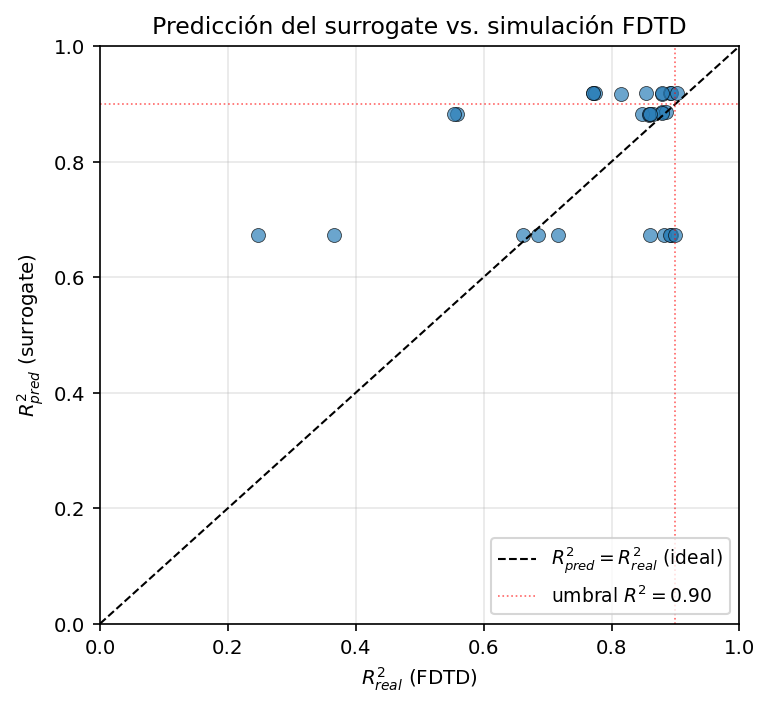
\includegraphics[width=0.55\textwidth]{Figuras/fig_pred_vs_real.png}
    \caption{Predicción del surrogate ($R^2_{\text{pred}}$) frente al valor real confirmado por FDTD ($R^2_{\text{real}}$) para los candidatos de las iteraciones 3--5. Los puntos por encima de la diagonal evidencian la sobreestimación del surrogate en la zona alta, que motivó la restricción al manifold.}
    \label{fig:pred_vs_real}
\end{figure}

La iteración~1 (GA libre) confirmó el diagnóstico de la Sección~\ref{subsec:ciclo_activo}: todos los candidatos colapsaron a $R^2 \approx 0.5$ con un \textit{gap} medio de $+0.48$ respecto a lo predicho. Al restringir al manifold (iter.~3--5), los candidatos se acercaron sistemáticamente al umbral: la iteración~4 produjo el primer cruce, \texttt{mvp\_c09} con $R^2_{\text{real}} = 0.9025$. La iteración~5, con la caja más estrecha ($5$~nm), no superó a la~4; de hecho, la mayoría de los candidatos derivados quedó por debajo de su \textit{seed}, indicando que las cuencas exploradas ya estaban cerca de su óptimo local.

\subsubsection{El \textit{Plateau} de las Iteraciones}

Tres iteraciones con cajas decrecientes ($20 \rightarrow 10 \rightarrow 5$~nm) y tres versiones del surrogate convergieron al mismo rango $[0.85, 0.91]$, sin que reducir la caja mejorara el resultado. Este \textit{plateau} resultó robusto al surrogate, al radio de búsqueda y a los \textit{seeds}, lo que sugería que el límite no era un defecto del modelo sino una propiedad del paisaje físico, una hipótesis que el análisis de cuencas confirmaría.

% --------------------------------------------------
\subsection{Convergencia del Pipeline: Calidad Global de los Candidatos}\label{subsec:convergencia}

Más allá del puñado de geometrías que cruzan el umbral $R^2 \geq 0.90$, el resultado agregado más informativo es el desplazamiento de toda la distribución de calidad de los candidatos respecto al muestreo aleatorio del diseño de experimentos. La Tabla~\ref{tab:convergencia} compara la distribución de $R^2_{\text{real}}$ del conjunto base (DoE) con la de los candidatos producidos por el enfoque definitivo: el GA restringido al manifold (iteraciones 3--5) y el hill-climbing sobre la cuenca robusta.

\begin{table}[H]
\centering
\small
\begin{tabular}{lccccc}
\toprule
\textbf{Conjunto} & \textbf{$n$} & \textbf{$R^2_{\text{real}}$ medio} & \textbf{$\geq 0.60$} & \textbf{$\geq 0.85$} & \textbf{$\geq 0.90$} \\
\midrule
DoE (conjunto base)                          & 1{,}110 & 0.24 & 11\,\% & 2.1\,\% & 0.4\,\% \\
GA restringido al manifold (iter.\ 3--5)     & 30      & 0.79 & 87\,\% & 60\,\%  & 3\,\%   \\
Hill-climbing cuenca robusta (627)           & 50      & 0.73 & 92\,\% & 18\,\%  & 6\,\%   \\
\bottomrule
\end{tabular}
\caption{Distribución de $R^2_{\text{real}}$ de los candidatos del enfoque definitivo frente al muestreo aleatorio del DoE. El enfoque definitivo concentra los candidatos en la región de alta calidad, desplazando la media de $0.24$ a ${\sim}0.79$.}
\label{tab:convergencia}
\end{table}

El contraste es drástico. Mientras que en el DoE solo el $11\%$ de las geometrías alcanza $R^2_{\text{real}} \geq 0.60$ y la media es $0.24$, los candidatos del GA restringido al manifold se concentran masivamente en la región de alta calidad: el $87\%$ supera $0.60$, el $60\%$ supera $0.85$ (frente a apenas $2.1\%$ en el DoE) y su $R^2$ medio es $0.79$, más del triple de la media del muestreo aleatorio. El hill-climbing sobre la cuenca robusta sostiene esa concentración ($92\%$ por encima de $0.60$). En total, el enfoque definitivo produjo cuatro geometrías con $R^2_{\text{real}} \geq 0.90$ (una del GA y tres del hill-climbing).

Este desplazamiento es, por sí mismo, uno de los resultados más relevantes del proyecto: demuestra que el pipeline no halló sus mejores diseños por azar, sino que el surrogate aprendió a dirigir la búsqueda hacia la región fértil del espacio y el GA la explotó de forma sistemática. La diferencia entre una tasa de acierto del $2.1\%$ por encima de $R^2 \geq 0.85$ (DoE) y del $60\%$ (GA restringido al manifold) cuantifica el valor del enfoque de aprendizaje sobre la exploración no dirigida.

% --------------------------------------------------
\subsection{Cuencas de Óptimos Independientes}\label{subsec:cuencas}

Una auditoría del conjunto de datos reveló que la región $R^2 \geq 0.90$ no es un único óptimo sino tres cuencas geométricamente independientes, separadas por distancias euclidianas $\ell_2 \approx 0.5$ en el espacio de diseño (Tabla~\ref{tab:cuencas}). El optimizador siempre había convergido a una sola de ellas (la de \texttt{sim\_627}) porque ahí se ubicaban sus \textit{seeds}. Las otras dos, incluyendo el máximo absoluto del conjunto de datos, nunca se habían explorado como semillas.

\begin{table}[H]
\centering
\small
\begin{tabular}{lcccl}
\toprule
\textbf{Cuenca} & \textbf{Semilla} & \textbf{$R^2_{\text{real}}$} & \textbf{$c_{2c}$ ($\mu$m)} & \textbf{Perfil} \\
\midrule
042 & \texttt{sim\_042} & 0.9579 & 0.234 & periódico ($w$ constante) \\
721 & \texttt{sim\_721} & 0.9246 & 0.207 & variable \\
627 & \texttt{sim\_627} & 0.9208 & 0.299 & variable \\
\bottomrule
\end{tabular}
\caption{Las tres cuencas con $R^2 \geq 0.90$ identificadas en el conjunto de datos, geométricamente independientes entre sí.}
\label{tab:cuencas}
\end{table}

Esta estructura se aprecia al proyectar las $1{,}110$ geometrías ($102$ dimensiones) a sus dos primeras componentes principales (Figura~\ref{fig:pca_espacio}), que ya capturan el $80\%$ de la varianza, evidencia de la baja dimensionalidad efectiva del diseño de experimentos (Sección~\ref{subsec:doe}). Se recurre a esta proyección lineal, y no a una técnica no lineal como t-SNE o UMAP, porque el argumento de separación entre cuencas descansa en las distancias euclidianas del espacio original, que el PCA preserva de forma aproximada y que las técnicas no lineales distorsionan en favor de la estructura local. La fracción de varianza capturada confirma, además, que la estructura relevante es de baja dimensión y mayormente lineal, por lo que una proyección no lineal no aportaría información adicional para este propósito. Las geometrías de alto $R^2$ no se dispersan por todo el espacio, sino que se concentran en regiones separadas, coherente con la noción de
\emph{manifold} (Sección~\ref{subsec:diseno_inverso}): los buenos enfocadores viven en una variedad de baja dimensión, y las tres cuencas ocupan zonas distintas de ella.

\begin{figure}[H]
    \centering
    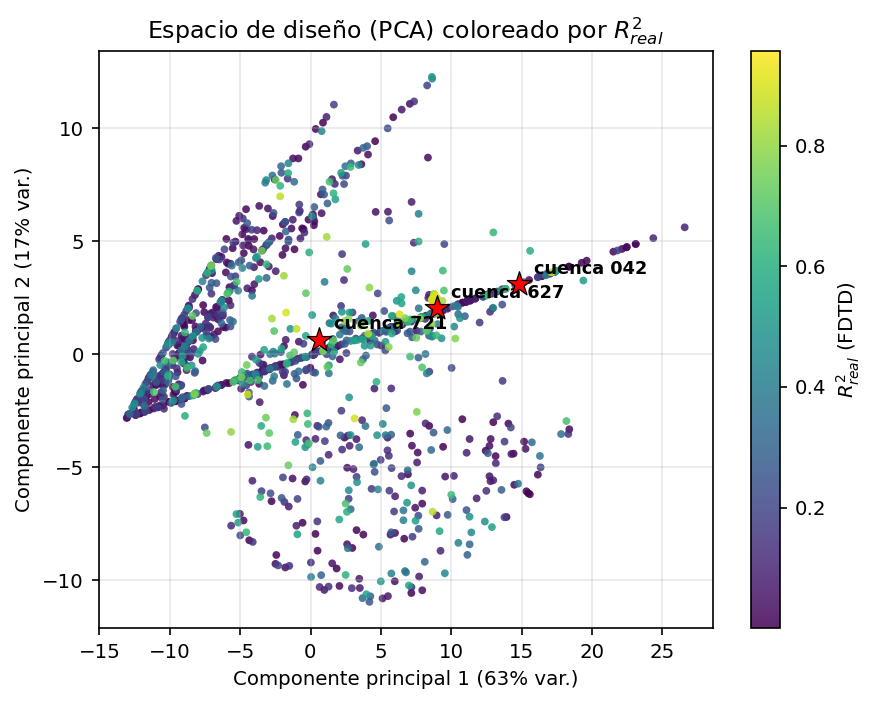
\includegraphics[width=0.74\textwidth]{Figuras/fig_pca_espacio.png}
    \caption{Proyección PCA (2~componentes, $80\%$ de varianza) de las $1{,}110$ geometrías
    del dataset, coloreadas por $R^2_{\text{real}}$. Las semillas de las tres cuencas
    (estrellas rojas) ocupan regiones geométricamente separadas; los enfocadores de alto
    $R^2$ se concentran en pocas zonas, no de forma uniforme.}
    \label{fig:pca_espacio}
\end{figure}

% --------------------------------------------------
\subsection{Hallazgo Central: Cuencas ``Aguja'' frente a ``Amplia''}\label{subsec:aguja_amplia}

Para caracterizar las tres cuencas se aplicó hill-climbing por FDTD directa
(Sección~\ref{subsec:hill_climbing}): $50$ perturbaciones gaussianas de $\sigma = 5$~nm por cuenca, validadas individualmente. La Tabla~\ref{tab:hill_climbing} resume los resultados, que revelan una diferencia cualitativa fundamental entre cuencas.

\begin{table}[H]
\centering
\small
\begin{tabular}{lccccc}
\toprule
\textbf{Cuenca} & \textbf{Tipo} & \textbf{Mejor $R^2_{\text{real}}$} & \textbf{$R^2_{\text{real}}$ medio} & \textbf{$N(\geq 0.90)$} & \textbf{$N(<0.70)$} \\
\midrule
627 & \textbf{amplia} & \textbf{0.9256} & 0.732 & 3 / 50 & 17 / 50 \\
042 & aguja & 0.7840 & 0.363 & 0 / 50 & 46 / 50 \\
721 & aguja & 0.7778 & 0.313 & 0 / 50 & 45 / 50 \\
\bottomrule
\end{tabular}
\caption{Resultados del hill-climbing FDTD ($50$ perturbaciones $\sigma=5$~nm por cuenca).
La cuenca 627 tolera las perturbaciones; las cuencas 042 y 721 colapsan.}
\label{tab:hill_climbing}
\end{table}

\begin{figure}[H]
    \centering
    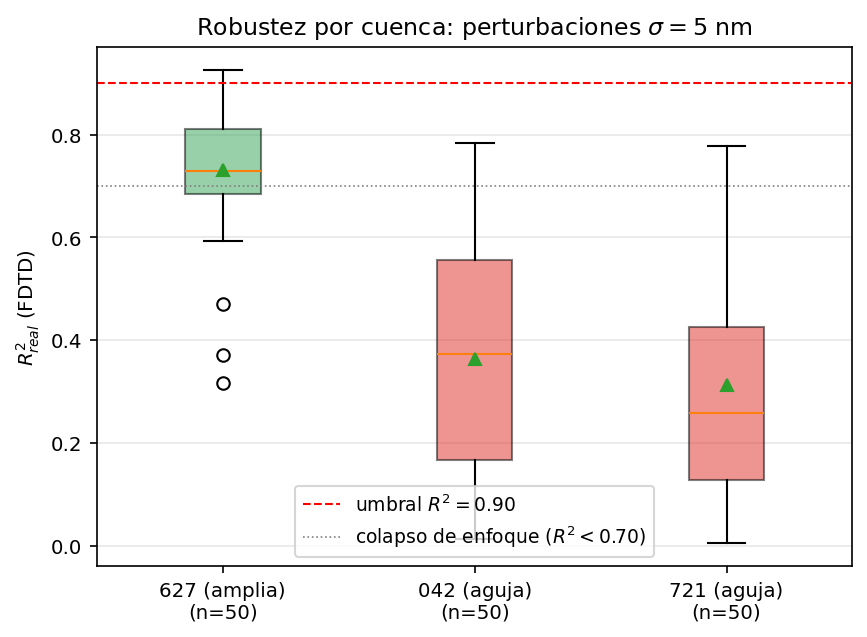
\includegraphics[width=0.72\textwidth]{Figuras/fig_cuencas_robustez.png}
    \caption{Distribución de $R^2_{\text{real}}$ bajo perturbaciones de $\sigma=5$~nm por cuenca. La cuenca amplia (627, verde) mantiene su distribución cerca del umbral; las cuencas aguja (042, 721, rojas) se dispersan muy por debajo del colapso de enfoque ($R^2 < 0.70$). El triángulo marca la media.}
    \label{fig:cuencas_robustez}
\end{figure}

Los contrastes son:

\begin{itemize}
    \item \textbf{Cuenca amplia (627)}: tolera
    perturbaciones de $\pm 5$~nm y el hill-climbing incluso mejoró el
    \textit{seed}, elevando el $R^2$ de $0.9025$ (\texttt{mvp\_c09}) a $0.9256$ (\texttt{hc627\_036}). Su $R^2$ medio bajo perturbación es $0.73$ y produjo tres geometrías con $R^2 \geq 0.90$.
    \item \textbf{Cuencas aguja (042, 721)}: pese a tener los máximos puntuales más altos del conjunto de datos ($0.9579$ y $0.9246$), son crestas extremadamente estrechas. El $90\%$ o más de las perturbaciones de $\pm 5$~nm degradan el $R^2$ por debajo de $0.70$, y ninguna alcanza siquiera $0.85$. El máximo histórico es inalcanzable con
    cualquier perturbación.

\end{itemize}

La implicación de ingeniería es directa: una tolerancia de fabricación litográfica del orden de $\pm 5$~nm destruye el enfoque en las cuencas aguja, mientras que la cuenca amplia lo conserva. El valor del pipeline ML no fue meramente cruzar el umbral $R^2 \geq 0.90$, sino localizar la cuenca robusta del paisaje, de mayor utilidad práctica que los máximos puntuales hallados por el muestreo aleatorio del diseño de experimentos. La Figura~\ref{fig:aguja_meseta} sintetiza el contraste de forma esquemática: una cuenca aguja alcanza un máximo más alto pero colapsa dentro de la banda de tolerancia de $\pm5$~nm, mientras que la meseta sacrifica algo de pico a cambio de mantener $R^2 \geq 0.85$ en toda esa banda.

\begin{figure}[H]
    \centering
    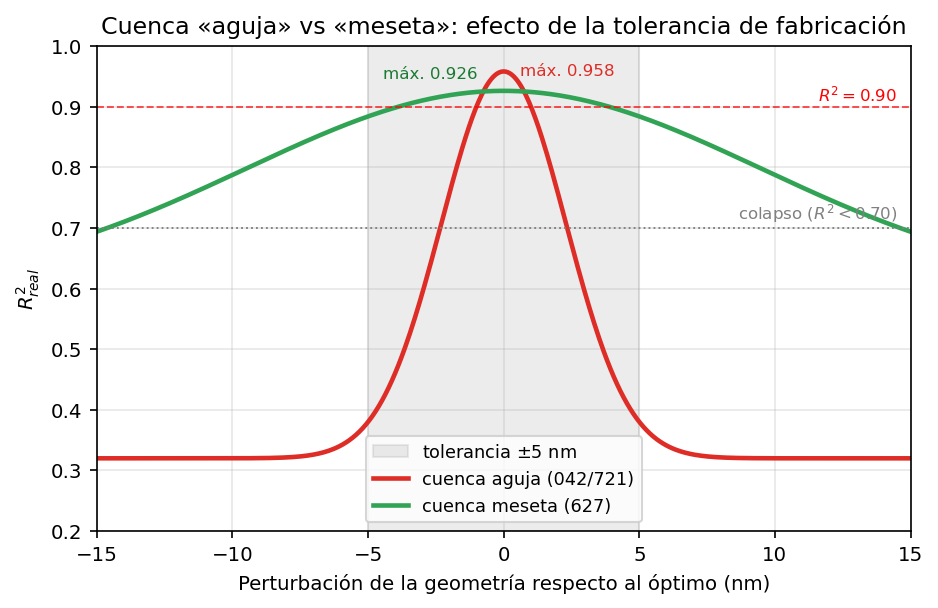
\includegraphics[width=0.74\textwidth]{Figuras/fig_aguja_meseta.png}
    \caption{Esquema del hallazgo central, anclado a los valores reales. La cuenca \emph{aguja} (042/721) alcanza un $R^2$ máximo más alto ($0.958$) pero su perfil es tan estrecho que la tolerancia de fabricación de $\pm5$~nm (banda gris) lo hunde por debajo del colapso de enfoque; la cuenca \emph{meseta} (627, máximo $0.926$) permanece por encima de $R^2 \approx 0.85$ en toda la banda. La robustez, no el máximo puntual, es lo
    que tiene valor de ingeniería.}
    \label{fig:aguja_meseta}
\end{figure}

% --------------------------------------------------
\subsection{Geometría Recomendada}\label{subsec:geometria_final}

La geometría recomendada como resultado del proyecto es \texttt{hc627\_036}, con $R^2_{\text{real}} = 0.9256$, por combinar alto rendimiento y robustez. Se acompaña de dos candidatos adicionales de la misma cuenca robusta, \texttt{hc627\_008} ($0.9134$) y \texttt{hc627\_043} ($0.9014$), que ofrecen alternativas de diseño con garantías similares de tolerancia a fabricación. La geometría se caracteriza por $c_{2c} = 0.300\;\mu$m y un perfil de anchos variable con media ${\sim}0.088\;\mu$m. El conjunto completo de candidatos ordenados se entrega en el repositorio de código (\texttt{results/final/}). La Figura~\ref{fig:perfil_hc627} muestra su perfil de anchos y la Figura~\ref{fig:campo_hc627} el perfil de intensidad resultante en el plano focal.

\begin{figure}[H]
    \centering
    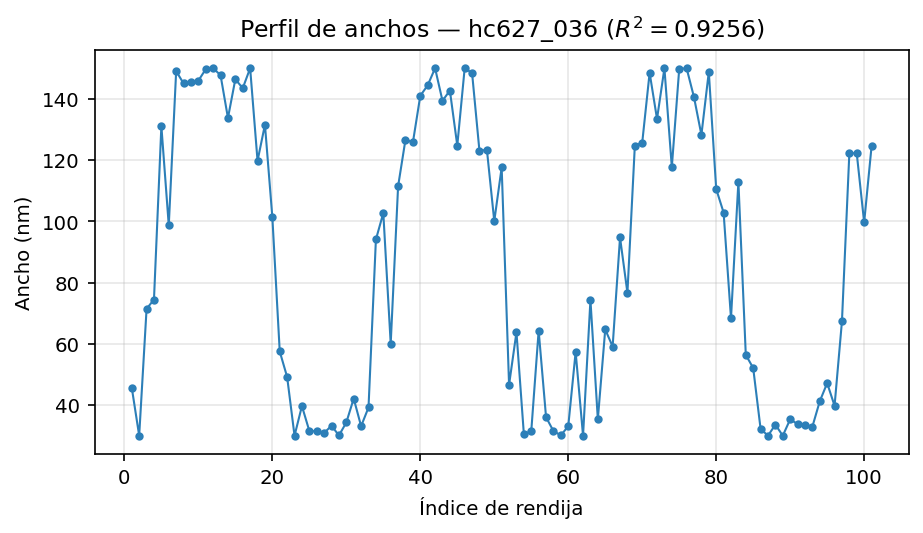
\includegraphics[width=0.8\textwidth]{Figuras/fig_perfil_hc627.png}
    \caption{Perfil de anchos de rendija de la geometría recomendada \texttt{hc627\_036}
    ($R^2_{\text{real}} = 0.9256$).}
    \label{fig:perfil_hc627}
\end{figure}

El perfil de anchos (Figura~\ref{fig:perfil_hc627}) es, en sí mismo, revelador: no es la parábola suave de una lente convergente clásica, sino un patrón oscilatorio cuasi-periódico, en el que los anchos alternan entre ${\sim}30$ y ${\sim}150$~nm a lo largo de unos cuatro lóbulos del arreglo. Es precisamente el tipo de configuración no intuitiva que un diseño analítico guiado por la intuición de lente difícilmente propondría y que el diseño inverso asistido por aprendizaje sí localiza: el enfoque emerge de una modulación distribuida y compleja de la fase, no de un gradiente monotónico de anchos.

\begin{figure}[H]
    \centering
    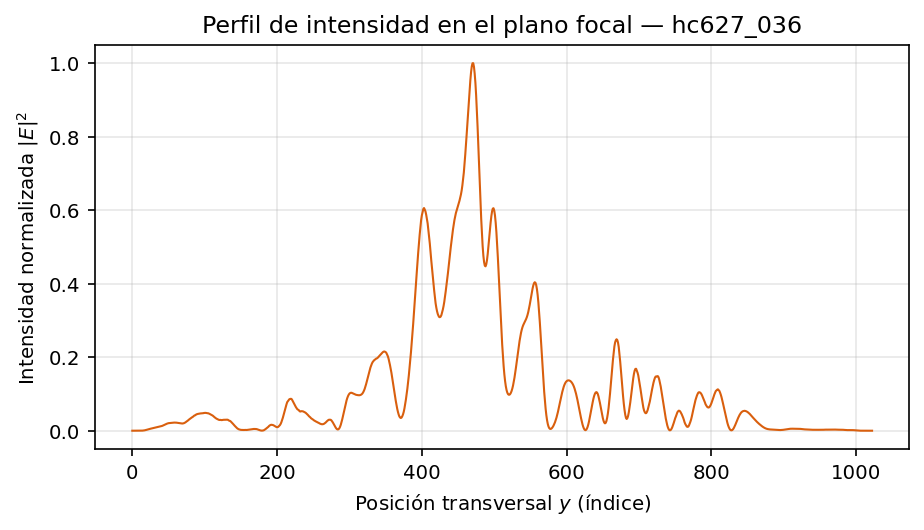
\includegraphics[width=0.8\textwidth]{Figuras/fig_campo_hc627.png}
    \caption{Perfil de intensidad normalizada $|E|^2$ en el plano focal de
    \texttt{hc627\_036}, obtenido por FDTD.}
    \label{fig:campo_hc627}
\end{figure}

El perfil de intensidad en el plano focal (Figura~\ref{fig:campo_hc627}) confirma el enfoque: la energía se concentra en un lóbulo central dominante, muy por encima de los lóbulos secundarios, en claro contraste con los perfiles anchos y planos de las configuraciones no enfocadoras caracterizadas en el EDA (Figura~\ref{fig:eda_campos}a). Es esta concentración transversal, sostenida a lo largo del eje de propagación, la que produce el ajuste parabólico con $R^2_{\text{real}} = 0.9256$ que define el criterio de éxito.

% --------------------------------------------------
\subsection{Eficiencia Computacional}\label{subsec:eficiencia}

La ventaja del enfoque subrogado en la fase de búsqueda es de varios órdenes de magnitud. La Tabla~\ref{tab:speedup} contrasta el costo de evaluar una geometría con FDTD frente al surrogate (medido en CPU sobre el modelo entrenado).

\begin{table}[H]
\centering
\small
\begin{tabular}{lcc}
\toprule
\textbf{Método} & \textbf{Tiempo por geometría} & \textbf{Aceleración} \\
\midrule
Simulación FDTD (Meep)        & ${\sim}1{,}820$ s ($30.3$ min) & $1\times$ \\
Surrogate (inferencia individual) & $0.71$ ms & ${\sim}2.6\times10^{6}$ \\
Surrogate (inferencia por lotes)  & $0.036$ ms/geom & ${\sim}5\times10^{7}$ \\
\bottomrule
\end{tabular}
\caption{Comparación del costo de evaluación por geometría. El tiempo FDTD proviene de los trabajos de confirmación reales ($18{,}200$ s para $10$ simulaciones); el del surrogate, de un \textit{benchmark} de inferencia.}
\label{tab:speedup}
\end{table}

La implicación a escala de pipeline es contundente: una ejecución del GA evalúa del orden de $2 \times 10^4$ geometrías (población $250 \times 80$ generaciones) en menos de un segundo con el surrogate. Explorar ese mismo número de geometrías por FDTD directa requeriría ${\sim}10{,}100$ horas de cómputo (${\sim}1.2$ años en un nodo). El costo de FDTD se reserva exclusivamente para la confirmación de los ${\sim}10$ candidatos finales de cada iteración y para el refinamiento por hill-climbing, manteniendo el presupuesto de simulación acotado a unas pocas horas por iteración. Esta reducción del costo computacional es precisamente el objetivo planteado en la propuesta del proyecto.

% --------------------------------------------------
\subsection{Comparación con Trabajos Previos}\label{subsec:comparacion}

Una comparación cuantitativa directa con la literatura no es posible en este problema, porque los trabajos afines difieren en el dominio físico, el objetivo óptico y la métrica reportada; no existe un \textit{benchmark} común de referencia. Procede, en cambio, una comparación metodológica, que sitúa las decisiones de diseño de este trabajo frente a las alternativas del estado del arte (Tabla~\ref{tab:comparacion}).

\begin{table}[H]
\centering
\footnotesize
\begin{tabular}{@{}>{\raggedright\arraybackslash}p{0.16\textwidth}
                  >{\raggedright\arraybackslash}p{0.19\textwidth}
                  >{\raggedright\arraybackslash}p{0.19\textwidth}
                  >{\raggedright\arraybackslash}p{0.16\textwidth}
                  >{\raggedright\arraybackslash}p{0.16\textwidth}@{}}
\toprule
\textbf{Trabajo} & \textbf{Dominio / objetivo} & \textbf{Método de aprendizaje} & \textbf{Optimización} & \textbf{Salida del modelo} \\
\midrule
Sosa-Sánchez y Téllez-Limón~\cite{airy_metalens} (referencia) & Metalente plasmónica de nano-rendijas (haz de Airy) & Ninguno: diseño analítico por \textit{phase matching} & Cierre analítico (dos anchos) & --- \\
\addlinespace
Liu \textit{et al.}~\cite{liu2018tandem} & Estructuras nanofotónicas (dispersión) & Red neuronal en tándem (inverso directo) & Inferencia directa del inverso & Geometría \\
\addlinespace
Maia \textit{et al.}~\cite{maia2025inverse} & Nanoestructuras plasmónicas & Ensambles (CatBoost, RF, Extra Trees) & Predicción directa de parámetros & Parámetro escalar (radio) \\
\addlinespace
Gao \textit{et al.}~\cite{gao2025surrogate} & Metasuperficies de bajo \textit{scattering} & Subrogado multi-característica & Evolución diferencial & Respuesta EM \\
\addlinespace
\textbf{Este trabajo} & Metalente plasmónica de nano-rendijas (enfoque) & MLP multi-salida del campo focal & GA restringido al manifold + hill-climbing FDTD & Campo complejo focal $|E|,\Phi$ \\
\bottomrule
\end{tabular}
\caption{Comparación metodológica con trabajos previos. El número de simulaciones de
entrenamiento varía en órdenes de magnitud entre enfoques (p.ej.\ ${\sim}1.4\times10^{5}$
en~\cite{maia2025inverse} frente a ${\sim}1{,}100$ en este trabajo).}
\label{tab:comparacion}
\end{table}

Del contraste se desprenden tres posicionamientos. Primero, frente al diseño inverso directo, en el que una red aprende el mapeo respuesta~$\rightarrow$~geometría y debe sortear la no-unicidad del problema, como en la arquitectura en tándem de~\cite{liu2018tandem}, este trabajo emplea un subrogado \textit{directo} (geometría $\rightarrow$ respuesta) acoplado a un optimizador, evitando así la patología de no-unicidad a costa de delegar la búsqueda al algoritmo genético. Segundo, frente a los modelos que predicen un escalar (un parámetro geométrico o una figura de mérito, como en~\cite{maia2025inverse}), aquí se predice el campo óptico focal completo, del que se deriva a posteriori cualquier métrica. Esta decisión, además, resultó esencial para evitar el desbalance que estancó el primer enfoque (Sección~\ref{sec:modelado}). Tercero, este trabajo comparte con~\cite{gao2025surrogate} la filosofía de acoplar un subrogado con un optimizador evolutivo, pero aporta dos elementos exigidos por la escasez de datos ($\sim$1{,}100 simulaciones en 102 dimensiones): la restricción al manifold de geometrías validadas, sin la cual el optimizador explota las regiones donde el subrogado extrapola, y la caracterización de robustez de las cuencas, que reveló el hallazgo central aguja/amplia (Sección~\ref{subsec:aguja_amplia}).

Respecto al trabajo de referencia~\cite{airy_metalens}, la diferencia es de naturaleza metodológica: aquel obtiene la geometría por un \textit{cierre analítico} del \textit{phase matching} (bastan dos anchos de rendija para reproducir el perfil de Airy objetivo), mientras que aquí la geometría se descubre mediante búsqueda inversa sobre el espacio completo de 101 anchos independientes. Ambos enfoques son complementarios y no comparables por su valor de $R^2$, pues optimizan objetivos ópticos distintos (generación de un haz de Airy con eficiencia de transmisión ${\sim}60\%$ en~\cite{airy_metalens}, frente a enfoque parabólico en este trabajo).

\subsubsection{Sobre el Conjunto Externo de la Investigadora}\label{subsubsec:consultora}

El proyecto dispuso de un conjunto adicional de $200$ simulaciones proporcionadas por la investigadora responsable (\texttt{Simulation\_XXX}), que se reservó como posible referencia externa (Sección~\ref{subsec:generacion}). Tras el análisis, se concluye que no constituye una comparación cuantitativa válida del modelo, por tres razones:

\begin{enumerate}
    \item \textbf{Incompatibilidad de la entrada.} El surrogate fija la dimensión de entrada en $102$ ($101$ anchos más la separación). Las geometrías de este conjunto emplean un número de rendijas distinto y variable (del orden de decenas a cientos), por lo que
    \emph{no son representables} en el espacio de entrada del modelo sin redefinir su parametrización. De hecho, los archivos disponibles conservan solo la respuesta óptica ($R^2$, fase, transmitancia), no el vector geométrico, lo que impide incluso construir la entrada.
    \item \textbf{Régimen físico fuera de distribución.} Aun reparametrizando, estas simulaciones operan en un régimen muy distinto del de entrenamiento: el plano focal abarca entre $383$ y ${\sim}10{,}400$ puntos transversales (media ${\sim}4{,}400$, frente a ${\sim}800$ en el conjunto propio), reflejo de dominios y aperturas mucho mayores y de separaciones centro a centro de hasta $0.70\;\mu$m. Cualquier predicción sería una extrapolación masiva, no una medida del desempeño del modelo en su dominio de diseño.
    \item \textbf{Propósito.} Por lo anterior, este conjunto se conserva únicamente como referencia externa cualitativa, evidencia de que existen buenos enfocadores en otros regímenes, con un máximo de $R^2 = 0.9956$ (\texttt{Simulation\_22}), y no como banco de prueba del surrogate. Evaluar la generalización fuera del régimen de $101$ rendijas exigiría un modelo con entrada de longitud variable, que se plantea como trabajo
    futuro (Sección~\ref{subsec:trabajo_futuro}).
\end{enumerate}
